\documentclass[notes,10pt, aspectratio=169]{beamer}

\usepackage{pgfpages}
% These slides also contain speaker notes. You can print just the slides,
% just the notes, or both, depending on the setting below. Comment out the want
% you want.
\setbeameroption{hide notes} % Only slide
%\setbeameroption{show only notes} % Only notes
%\setbeameroption{show notes on second screen=right} % Both
\usepackage{colortbl}
\usepackage{helvet}
\usepackage[default]{lato}
\usepackage{array}
\usepackage{eurosym}
\usepackage{setspace}
\usepackage{animate}
\usepackage{multicol}
\usepackage{breqn}
\usepackage{subcaption}
\usepackage{caption}
\captionsetup{font=scriptsize, justification=raggedright,singlelinecheck=false}
\usepackage[export]{adjustbox}
\usepackage[scale=2]{ccicons}
\usepackage{tikz}
\newenvironment{wideitemize}{\itemize\addtolength{\itemsep}{10pt}}{\enditemize}
\usepackage{natbib}

\usepackage{tikz}
\usepackage{verbatim}
\setbeamertemplate{note page}{\pagecolor{yellow!5}\insertnote}
\usepackage{amsmath}
%\usepackage{mathpazo}
\usepackage{hyperref}
\usepackage{lipsum}
\usepackage{multimedia}
\usepackage{multirow}
\usepackage{graphicx}
\usepackage{dcolumn}
\usepackage{bbm}
\newcolumntype{d}[0]{D{.}{.}{5}}

\usepackage{changepage}
\usepackage{appendixnumberbeamer}
% \newcommand{\beginbackup}{
%   \newcounter{framenumbervorappendix}
%   \setcounter{framenumbervorappendix}{\value{framenumber}}
%   \setbeamertemplate{footline}
%   {
%      \leavevmode%
%      \hline
%      box{%
%       \begin{beamercolorbox}[wd=\paperwidth,ht=2.25ex,dp=1ex,right]{footlinecolor}%
% %         \insertframenumber  \hspace*{2ex} 
%       \end{beamercolorbox}}%
%      \vskip0pt%
%   }
%  }

 \setbeamertemplate{footline}{
    \hbox{%
    \begin{beamercolorbox}[wd=\paperwidth,ht=3ex,dp=1.5ex,leftskip=2ex,rightskip=2ex]{page footer}%
        %\usebeamerfont{title in head/foot}%
        %\insertshorttitle \hfill
        %\insertsection \hfill
        %\tableofcontents[currentsection] \hfill
        \insertsectionnavigationhorizontal{0.7\paperwidth}{}{} \hfill 
        \insertframenumber{} / \inserttotalframenumber
    \end{beamercolorbox}}%
}
\newcommand{\backupend}{
   \addtocounter{framenumbervorappendix}{-\value{framenumber}}
   \addtocounter{framenumber}{\value{framenumbervorappendix}} 
}

\useinnertheme[shadow]{rounded}
\setbeamercolor{block title example}{fg=black,bg=orange!50!white}
\setbeamercolor{block body example}{fg=black, bg=orange!30!white}
\setbeamercolor{block title alert}{fg=black,bg=green!50!white}
\setbeamercolor{block body alert}{fg=black, bg=green!30!white}
\setbeamercolor{block title}{use=structure,fg=structure.fg,bg=structure.fg!20!bg}
\setbeamercolor{block body}{parent=normal text,use=block title,bg=block title.bg!50!bg}

\newcommand\independent{\protect\mathpalette{\protect\independenT}{\perp}}
\def\independenT#1#2{\mathrel{\rlap{$#1#2$}\mkern2mu{#1#2}}}

\usepackage{graphicx}
\usepackage[space]{grffile}
\usepackage{booktabs}

% These are my colors -- there are many like them, but these ones are mine.
\definecolor{blue}{RGB}{0,114,178}
\definecolor{red}{RGB}{213,94,0}
\definecolor{yellow}{RGB}{240,228,66}
\definecolor{green}{RGB}{0,158,115}

\setbeamercolor{section in head/foot}{fg=blue}


\hypersetup{
  colorlinks=false,
  linkbordercolor = {white},
  linkcolor = {blue}
}


%% I use a beige off white for my background
\definecolor{MyBackground}{RGB}{255,253,218}

%% Uncomment this if you want to change the background color to something else
%\setbeamercolor{background canvas}{bg=MyBackground}

%% Change the bg color to adjust your transition slide background color!
\newenvironment{transitionframe}{
  \setbeamercolor{background canvas}{bg=yellow}
  \begin{frame}}{
    \end{frame}
}

\setbeamercolor{frametitle}{fg=blue}
\setbeamercolor{title}{fg=black}
%\setbeamertemplate{footline}[frame number]
\setbeamertemplate{navigation symbols}{} 
\setbeamertemplate{itemize items}{-}
\setbeamercolor{itemize item}{fg=blue}
\setbeamercolor{itemize subitem}{fg=blue}
\setbeamercolor{enumerate item}{fg=blue}
\setbeamercolor{enumerate subitem}{fg=blue}
\setbeamercolor{button}{bg=white,fg=blue,}



% If you like road maps, rather than having clutter at the top, have a roadmap show up at the end of each section 
% (and after your introduction)
% Uncomment this is if you want the roadmap!
% \AtBeginSection[]
% {
%    \begin{frame}
%        \frametitle{Roadmap of Talk}
%        \tableofcontents[currentsection]
%    \end{frame}
% }
\setbeamercolor{section in toc}{fg=blue}
\setbeamercolor{subsection in toc}{fg=red}
%\setbeamersize{text margin left=1em,text margin right=1em} 
\setbeamersize{text margin left=0.7cm,text margin right=0.7cm} 


\title[]{\textcolor{blue}{Lecture 9 v2:\\An Introduction to Instrumental Variables}}
\author{25117 - Econometrics}
\institute[shortinst]{Universitat Pompeu Fabra}

\date{November 18th, 2024}

\begin{document}

\begin{frame}[plain]
\maketitle
\end{frame}



\begin{frame}{What we learned in the last lesson}
\begin{itemize}
    \item Statistical studies are evaluated by asking whether the analysis is internally and externally valid.\\[1em]
    \item A study is internally valid if the statistical inferences about causal effects are valid for the population being studied. In regression estimation of causal effects, there are two main types of threats to internal validity:
    \begin{itemize}
        \item First, OLS estimators are biased and inconsistent if the regressors and error terms are correlated.
        \item Second, confidence intervals and hypothesis tests are not valid when the standard errors are incorrect.
    \end{itemize}
    \vspace{1em}
    \item A study is externally valid if its inferences and conclusions can be generalized from the population and setting studied to other populations and settings.
\end{itemize} 
\end{frame}


\begin{frame}{Instrumental Variables}
Consider the following regression model:
\begin{equation*}
    Y_i = \beta_0 + \beta_1 X_i + u_i
\end{equation*}
\begin{itemize}
    \item OVB,  Simultaneous causality bias, Errors-in-variables bias... all three result in $\mathbb{E}(u\mid X)\neq0$\\[1em]
    \item Instrumental variables regression can eliminate bias when $\mathbb{E}(u\mid X)\neq0$, using an instrumental variable (IV), $Z$.\\[1em]
    \item Intuitively, IV regression breaks $X$ into two parts:
    \begin{enumerate}
        \item an \textit{endogenous} part that might be correlated with $u$, and 
        \item an \textit{exogenous}  part that is not. 
    \end{enumerate}
    \vspace{1em}
By isolating the part that is not correlated with $u$, it is possible to estimate $\beta_1$
\end{itemize}
\end{frame}



\begin{frame}{Instrumental Variables}
For an instrumental variable (an “instrument”) Z to be valid, it must satisfy two conditions:
\begin{enumerate}
    \item \textbf{Instrument relevance:} $Z$ is a strong determinant of $X$ ($corr(Z, X)\neq 0$)
    \item \textbf{Instrument exogeneity (exclusion restriction):} $Z$ is unrelated to $u$ ($corr(Z, u) = 0$)
\end{enumerate}

\begin{center}
\begin{figure}
    \resizebox{.9\linewidth}{!}{%

\tikzset{every picture/.style={line width=0.75pt}} %set default line width to 0.75pt        

\begin{tikzpicture}[x=0.75pt,y=0.75pt,yscale=-1,xscale=1]
%uncomment if require: \path (0,292); %set diagram left start at 0, and has height of 292

%Shape: Ellipse [id:dp6518310746416693] 
\draw   (187.23,223.93) .. controls (187.23,206.77) and (201.01,192.85) .. (218,192.85) .. controls (234.99,192.85) and (248.77,206.77) .. (248.77,223.93) .. controls (248.77,241.09) and (234.99,255) .. (218,255) .. controls (201.01,255) and (187.23,241.09) .. (187.23,223.93) -- cycle ;
%Shape: Ellipse [id:dp21717165537664984] 
\draw   (556.46,222.68) .. controls (556.46,205.52) and (570.24,191.61) .. (587.23,191.61) .. controls (604.22,191.61) and (618,205.52) .. (618,222.68) .. controls (618,239.85) and (604.22,253.76) .. (587.23,253.76) .. controls (570.24,253.76) and (556.46,239.85) .. (556.46,222.68) -- cycle ;
%Shape: Ellipse [id:dp6180865660156953] 
\draw   (358.31,66.07) .. controls (358.31,48.91) and (372.08,35) .. (389.08,35) .. controls (406.07,35) and (419.85,48.91) .. (419.85,66.07) .. controls (419.85,83.23) and (406.07,97.15) .. (389.08,97.15) .. controls (372.08,97.15) and (358.31,83.23) .. (358.31,66.07) -- cycle ;
%Shape: Ellipse [id:dp049861641718563554] 
\draw  [color={rgb, 255:red, 11; green, 8; blue, 234 }  ,draw opacity=1 ] (42,84.72) .. controls (42,67.56) and (55.78,53.64) .. (72.77,53.64) .. controls (89.76,53.64) and (103.54,67.56) .. (103.54,84.72) .. controls (103.54,101.88) and (89.76,115.79) .. (72.77,115.79) .. controls (55.78,115.79) and (42,101.88) .. (42,84.72) -- cycle ;
%Straight Lines [id:da038069870660455196] 
\draw [color={rgb, 255:red, 6; green, 20; blue, 244 }  ,draw opacity=1 ] [dash pattern={on 4.5pt off 4.5pt}]  (94.92,107.09) -- (192.48,203.18) ;
\draw [shift={(194.62,205.28)}, rotate = 224.57] [fill={rgb, 255:red, 6; green, 20; blue, 244 }  ,fill opacity=1 ][line width=0.08]  [draw opacity=0] (8.93,-4.29) -- (0,0) -- (8.93,4.29) -- cycle    ;
%Straight Lines [id:da7311874040313404] 
\draw [color={rgb, 255:red, 244; green, 6; blue, 31 }  ,draw opacity=1 ] [dash pattern={on 4.5pt off 4.5pt}]  (361.09,88.06) -- (243.53,203.18) ;
\draw [shift={(241.38,205.28)}, rotate = 315.6] [fill={rgb, 255:red, 244; green, 6; blue, 31 }  ,fill opacity=1 ][line width=0.08]  [draw opacity=0] (8.93,-4.29) -- (0,0) -- (8.93,4.29) -- cycle    ;
\draw [shift={(363.23,85.96)}, rotate = 135.6] [fill={rgb, 255:red, 244; green, 6; blue, 31 }  ,fill opacity=1 ][line width=0.08]  [draw opacity=0] (8.93,-4.29) -- (0,0) -- (8.93,4.29) -- cycle    ;
%Straight Lines [id:da7673731200325982] 
\draw [color={rgb, 255:red, 126; green, 211; blue, 33 }  ,draw opacity=1 ]   (248.77,223.93) -- (553.46,222.7) ;
\draw [shift={(556.46,222.68)}, rotate = 179.77] [fill={rgb, 255:red, 126; green, 211; blue, 33 }  ,fill opacity=1 ][line width=0.08]  [draw opacity=0] (8.93,-4.29) -- (0,0) -- (8.93,4.29) -- cycle    ;
%Straight Lines [id:da44429091772583584] 
\draw [color={rgb, 255:red, 61; green, 222; blue, 2 }  ,draw opacity=1 ]   (414,84) -- (562.71,199.71) ;
\draw [shift={(565.08,201.55)}, rotate = 217.89] [fill={rgb, 255:red, 61; green, 222; blue, 2 }  ,fill opacity=1 ][line width=0.08]  [draw opacity=0] (8.93,-4.29) -- (0,0) -- (8.93,4.29) -- cycle    ;
%Curve Lines [id:da5510041670949384] 
\draw  [dash pattern={on 0.84pt off 2.51pt}]  (328,124) .. controls (400.64,233.45) and (560.39,197.37) .. (530.47,89.63) ;
\draw [shift={(530,88)}, rotate = 73.64] [color={rgb, 255:red, 0; green, 0; blue, 0 }  ][line width=0.75]    (10.93,-3.29) .. controls (6.95,-1.4) and (3.31,-0.3) .. (0,0) .. controls (3.31,0.3) and (6.95,1.4) .. (10.93,3.29)   ;
%Curve Lines [id:da9877608396858246] 
\draw  [dash pattern={on 0.84pt off 2.51pt}]  (463,120) .. controls (457.06,122.97) and (548.15,150.44) .. (530.57,89.86) ;
\draw [shift={(530,88)}, rotate = 72.39] [color={rgb, 255:red, 0; green, 0; blue, 0 }  ][line width=0.75]    (10.93,-3.29) .. controls (6.95,-1.4) and (3.31,-0.3) .. (0,0) .. controls (3.31,0.3) and (6.95,1.4) .. (10.93,3.29)   ;
%Curve Lines [id:da31587639785238864] 
\draw  [dash pattern={on 0.84pt off 2.51pt}]  (80.14,51.79) .. controls (98.88,16.95) and (120.26,40.2) .. (133,50) ;
\draw [shift={(79,54)}, rotate = 296.57] [color={rgb, 255:red, 0; green, 0; blue, 0 }  ][line width=0.75]    (10.93,-3.29) .. controls (6.95,-1.4) and (3.31,-0.3) .. (0,0) .. controls (3.31,0.3) and (6.95,1.4) .. (10.93,3.29)   ;

% Text Node
\draw (66,75) node [anchor=north west][inner sep=0.75pt]  [color={rgb, 255:red, 13; green, 16; blue, 187 }  ,opacity=1 ] [align=left] {$Z$};
% Text Node
\draw (212,217.29) node [anchor=north west][inner sep=0.75pt]   [align=left] {$X$};
% Text Node
\draw (580.23,214.05) node [anchor=north west][inner sep=0.75pt]   [align=left] {$Y$};
% Text Node
\draw (383,60) node [anchor=north west][inner sep=0.75pt]   [align=left] {$u$};
% Text Node
\draw (489,69) node [anchor=north west][inner sep=0.75pt]   [align=left] {$\mathbb{E}(u\mid X)\neq0$};
% Text Node
\draw (113,53) node [anchor=north west][inner sep=0.75pt]   [align=left] {Instrumental Variable (IV)};


\end{tikzpicture}
}
\end{figure}
\end{center}

\end{frame}




\begin{frame}{First Stage and Reduced Form}
The structural equation is $Y_i=\beta_0+\beta_1X_i+U_i$. Our goal is to recover the causal slope $\beta_1$ using the instrument $Z_i$.

\medskip
\textbf{First stage.} Regress $X_i$ on $Z_i$ with an intercept. The population slope $\pi_1$ measures how much $X_i$ changes in the fitted line per unit of $Z_i$.
\[
\pi_1=\frac{\operatorname{Cov}(Z_i,X_i)}{\operatorname{Var}(Z_i)}.
\]
\textbf{Reduced form (RF).} Regress $Y_i$ on $Z_i$ with an intercept. The population slope $\beta_1^{\mathrm{RF}}$ measures how much $Y_i$ changes in the fitted line per unit of $Z_i$.
\[
\beta_1^{\mathrm{RF}}=\frac{\operatorname{Cov}(Z_i,Y_i)}{\operatorname{Var}(Z_i)}.
\]
\end{frame}

\begin{frame}{How the Reduced Form Contains the Causal Slope}
Substitute the structural equation for $Y_i$ and expand the covariance.
\[
\begin{aligned}
\operatorname{Cov}(Z_i,Y_i)
&=\operatorname{Cov}(Z_i,\beta_0+\beta_1 X_i+U_i)\\
&=\underbrace{\operatorname{Cov}(Z_i,\beta_0)}_{0\text{ because }\beta_0\text{ is constant}}
+\beta_1\operatorname{Cov}(Z_i,X_i)
+\underbrace{\operatorname{Cov}(Z_i,U_i)}_{0\text{ by instrument exogeneity}}\\
&=\beta_1\operatorname{Cov}(Z_i,X_i).
\end{aligned}
\]
Divide both sides by $\operatorname{Var}(Z_i)$ to express the relationship in regression slopes.
\[
\underbrace{\frac{\operatorname{Cov}(Z_i,Y_i)}{\operatorname{Var}(Z_i)}}_{\beta_1^{\mathrm{RF}}}
=\beta_1\underbrace{\frac{\operatorname{Cov}(Z_i,X_i)}{\operatorname{Var}(Z_i)}}_{\pi_1}.
\]
The change in fitted $Y$ per unit of $Z$ equals the change in fitted $X$ per unit of $Z$ times the causal effect per unit of $X$.
\end{frame}

\begin{frame}{The IV Slope Is a Ratio}
Instrument relevance means $\operatorname{Cov}(Z_i,X_i)\neq0$, so the first-stage slope $\pi_1$ is nonzero. Divide $\beta_1^{\mathrm{RF}}=\beta_1\pi_1$ by $\pi_1$.
\[
\beta_1=\frac{\beta_1^{\mathrm{RF}}}{\pi_1}
=\frac{\operatorname{Cov}(Z_i,Y_i)/\operatorname{Var}(Z_i)}
      {\operatorname{Cov}(Z_i,X_i)/\operatorname{Var}(Z_i)}
=\frac{\operatorname{Cov}(Z_i,Y_i)}{\operatorname{Cov}(Z_i,X_i)}.
\]
For example, if a one-unit increase in $Z$ predicts a two-unit increase in $X$ and a six-unit increase in $Y$, the IV slope is $6/2=3$ units of $Y$ per unit of $X$.

\medskip
In the sample, the IV estimate is the \textbf{estimated reduced-form slope divided by the estimated first-stage slope}.
\[
\hat\beta_1^{\mathrm{IV}}
=\frac{\hat\beta_1^{\mathrm{RF}}}{\hat\pi_1}
=\frac{s_{ZY}/s_{ZZ}}{s_{ZX}/s_{ZZ}}
=\frac{s_{ZY}}{s_{ZX}},\text{ provided }s_{ZX}\ne0.
\]
As sample covariances converge to their population values, $\hat\beta_1^{\mathrm{IV}}\xrightarrow{p}\beta_1$.
\end{frame}

\begin{frame}{How Two-Stage Least Squares Computes the IV Slope}
\small
\setlength{\abovedisplayskip}{4pt}
\setlength{\belowdisplayskip}{4pt}
\begin{enumerate}
    \item Regress $X_i$ on $Z_i$ with an intercept. The predicted values are $\hat X_i=\hat\pi_0+\hat\pi_1 Z_i$, where $\hat\pi_1=s_{ZX}/s_{ZZ}$.
    \item Regress $Y_i$ on $\hat X_i$ with an intercept. Its slope is the 2SLS estimate.
\end{enumerate}
\medskip
Centering $\hat X_i=\hat\pi_0+\hat\pi_1 Z_i$ gives
$\hat X_i-\overline{\hat X}=\hat\pi_1(Z_i-\bar Z)$. Substitute into the sample covariance and variance.
\[
\begin{aligned}
s_{\hat X Y}
&=\frac{1}{n}\sum_{i=1}^{n}(\hat X_i-\overline{\hat X})(Y_i-\bar Y)
=\hat\pi_1\frac{1}{n}\sum_{i=1}^{n}(Z_i-\bar Z)(Y_i-\bar Y)
=\hat\pi_1s_{ZY},\\
s_{\hat X\hat X}
&=\frac{1}{n}\sum_{i=1}^{n}(\hat X_i-\overline{\hat X})^2
=\hat\pi_1^2\frac{1}{n}\sum_{i=1}^{n}(Z_i-\bar Z)^2
=\hat\pi_1^2s_{ZZ}.
\end{aligned}
\]
The second-stage OLS slope is therefore
\[
\hat\beta_1^{\mathrm{2SLS}}
=\frac{s_{\hat X Y}}{s_{\hat X\hat X}}
=\frac{\hat\pi_1 s_{ZY}}{\hat\pi_1^2s_{ZZ}}
=\frac{s_{ZY}}{\hat\pi_1s_{ZZ}}
=\frac{s_{ZY}}{s_{ZX}}.
\]
With one instrument and one endogenous regressor, two-stage least squares is another way to compute the same IV estimate of $\beta_1$, equal to the estimated reduced-form slope divided by the estimated first-stage slope: $\hat\beta_1^{\mathrm{2SLS}}=\hat\beta_1^{\mathrm{IV}}=\hat\beta_1^{\mathrm{RF}}/\hat\pi_1$.
\end{frame}

\begin{frame}{Two Stages Least Squares (2SLS)}
For another way to see it, consider the system of reduced-form equations:
\begin{eqnarray*}
    & X_i &= \pi_0 + \pi_1 Z_i + v_i\\
    & Y_i &= \gamma_0 + \gamma_1 Z_i + w_i
\end{eqnarray*}
Because $Z$ is exogenous, $Z$ is uncorrelated with both $v_i$ and $w_i$.\\[1em]
\underline{\textbf{The idea:}} An exogenous unit change in $Z$ results in a change in $X$ by $\pi_1$ units and a change in $Y$ by $\gamma_1$ units.\\[1em]

Thus an exogenous change in  $X$ by $\pi_1$ is associated with an exogenous change in $Y$ by $\gamma_1$ units.\\[1em]

So the effect on $Y$ of an exogenous change in $X$ is $\beta_1^{2SLS} = \gamma_1/\pi_1$
\end{frame}

\begin{frame}{A Buttery Example}
IV regressions were first developed in 1928 by Philip G. Wright to estimate supply and demand elasticities for agricultural goods,in particular, butter.\\[1em]

Consider the following demand equation:
\begin{equation*}
    ln(Q^{butter}_i) = \beta_0 + \beta_1 ln(P^{butter}_i)+ u_i
\end{equation*}
Here, $\beta_1$ captures the price-elasticity of butter, i.e., the percentage change in quantities due to a 1\% change in price.\\[1em]

\textbf{\underline{Problem:}} The OLS regression of $ln(Q^{butter}_i)$ on $ln(P^{butter}_i)$ suffers from simultaneity (reverse causality) bias.\\[1em]

Because prices, $ln(P^{butter}_i)$, are simultaneously determined in equilibrium by the interplay of supply and demand, $\beta_1$ was unlikely to capture neither the supply or demand elasticity of butter.

\end{frame}


\begin{frame}{A Buttery Example}
 \begin{columns}
\begin{column}{0.35\textwidth}
    \begin{itemize}
        \item In every period, prices are determined in equilibrium by the simultaneous movements of supply and demand 
        \item The equilibrium is determined by the intersection of the demand curve $D_k$ and supply curve $S_k$  
    \end{itemize}
\end{column}
\begin{column}{0.7\textwidth}
\begin{figure}
  \centering
         \vspace{-1mm}
        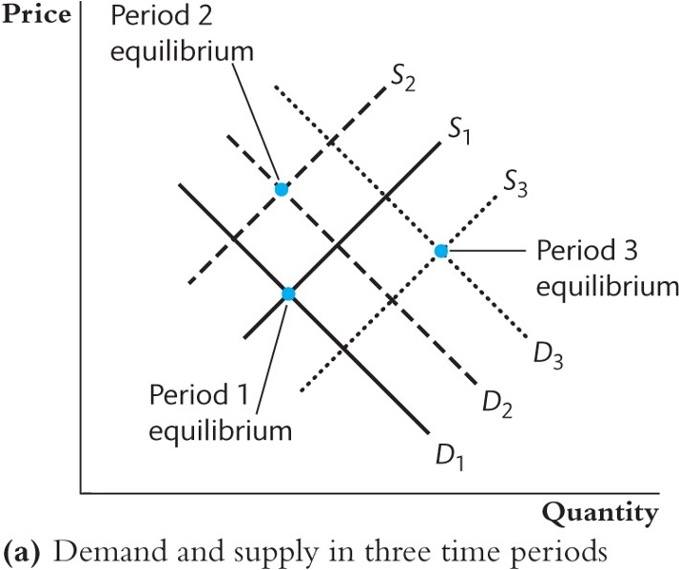
\includegraphics[scale=.35]{images/butter1.jpg}
\end{figure}
\end{column}
\end{columns}
\end{frame}

\begin{frame}{A Buttery Example}
 \begin{columns}
\begin{column}{0.35\textwidth}
    \begin{itemize}
        \item As a result, the set of $\{Price_k, Quantity_k\}$ is not informative about the specific demand and supply elasticities (i.e., the curves' slopes)
        \item In this example, demand and supply elasticities could be anything, from perfectly elastic (a small change in $P$ is associated with a high change in $Q$) to completely inelastic (a high change in $P$ is associated with a little change in $Q$).
    \end{itemize}
\end{column}
\begin{column}{0.7\textwidth}
\begin{figure}
  \centering
         \vspace{-1mm}
        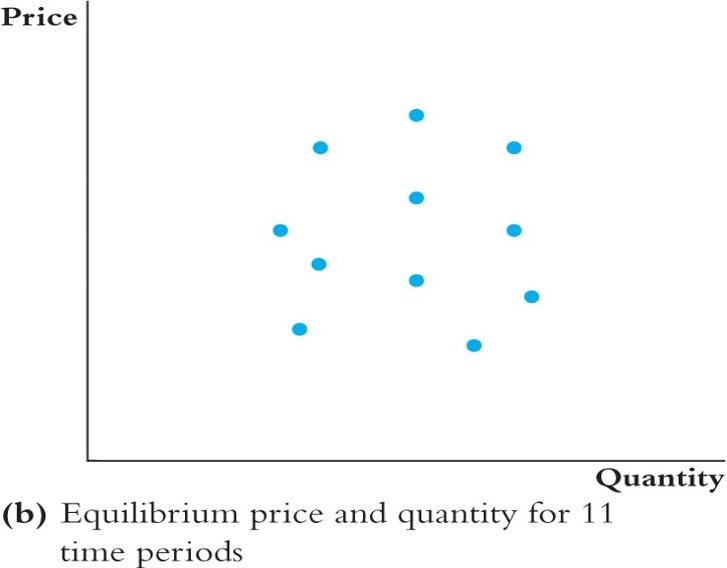
\includegraphics[scale=.35]{images/butter2.jpg}
\end{figure}
\end{column}
\end{columns}
\end{frame}

\begin{frame}{A Buttery Example}
 \begin{columns}
\begin{column}{0.35\textwidth}
    \begin{itemize}
        \item To determine the elasticity of demand, we need an IV that would shift only supply curves while leaving demand curves unchanged.
        \item What could be such an instrument?
    \end{itemize}
\end{column}
\begin{column}{0.7\textwidth}
\begin{figure}
  \centering
         \vspace{-1mm}
        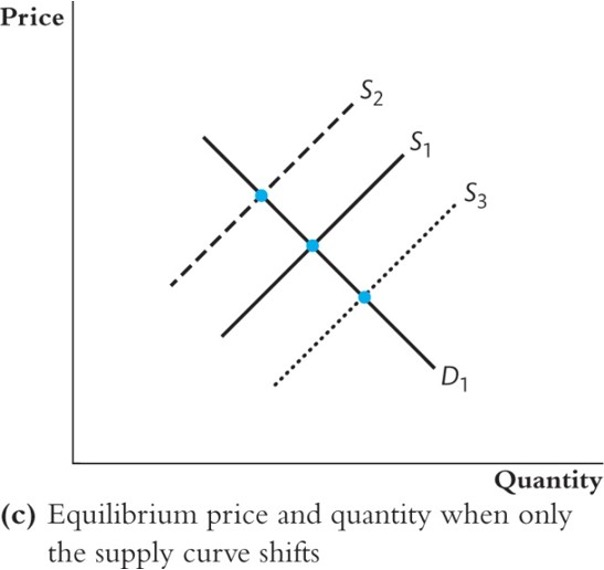
\includegraphics[scale=.35]{images/butter3.jpg}
\end{figure}
\end{column}
\end{columns}
\end{frame}

\begin{frame}{A Buttery Example}
A potential IV for the butter prices to estimate the demand elasticity for butter could be drought shocks to dairy regions ($Z$).\\[1em]
It is a plausibly revelant IV: below-average rainfall in a dairy region  ($Z$) could impair grazing and thus reduce butter production at a given price, shifting the supply curve to the left and increasing the equilibrium price  ($X$)\\[1em]
In this example, the drought shifts the supply curve left and leaves the demand curve unchanged. The higher equilibrium price leads to a movement along the demand curve, reducing the quantity of butter demanded.
\end{frame}

\begin{frame}{Large-Sample IV\texorpdfstring{ -- }{ - }Step 1: Write the Estimation Error}
Use the structural equation $Y_i=\beta_0+\beta_1X_i+U_i$.
\[
\begin{aligned}
s_{ZY}
&=\frac{1}{n}\sum_{i=1}^{n}(Z_i-\bar Z)(Y_i-\bar Y)\\
&=\frac{1}{n}\sum_{i=1}^{n}(Z_i-\bar Z)
  \bigl[\beta_1(X_i-\bar X)+(U_i-\bar U)\bigr]\\
&=\beta_1s_{ZX}+s_{ZU}.
\end{aligned}
\]
Substitute this into the IV ratio and subtract the true slope.
\[
\hat\beta_1^{\mathrm{IV}}-\beta_1
=\frac{\beta_1s_{ZX}+s_{ZU}}{s_{ZX}}-\beta_1
=\frac{s_{ZU}}{s_{ZX}}.
\]
\end{frame}

\begin{frame}{Step 2: Start from the Central Limit Theorem}
Suppose $W_1,\ldots,W_n$ are independent and identically distributed (i.i.d.), with mean $\mu_W$ and finite variance $\sigma_W^2$.
\[
\bar W=\frac{1}{n}\sum_{i=1}^{n}W_i,\text{ and }
\sqrt n\,(\bar W-\mu_W)
\xrightarrow{d}\mathcal N(0,\sigma_W^2).
\]
\begin{itemize}
    \item $\bar W-\mu_W$ is the sampling error of the average.
    \item The average fluctuates around $\mu_W$ on the $1/\sqrt n$ scale.
    \item Multiplication by $\sqrt n$ keeps these fluctuations on a stable scale.
    \item $\xrightarrow{d}$ means convergence in distribution. The scaled sampling error has a limiting normal distribution.
\end{itemize}
\medskip
To use the theorem for IV, we must identify the random variable $W_i$ whose average appears in the estimation error.
\end{frame}

\begin{frame}{Step 3: Identify the Variable We Average}
Let $\mu_Z=\mathbb E(Z_i)$ and absorb the mean of $U_i$ into the intercept so that $\mathbb E(U_i)=0$. Define
\[
W_i=(Z_i-\mu_Z)U_i.
\]
I.i.d. observations $(Z_i,U_i)$ give i.i.d. products $W_i$. Instrument exogeneity implies
\[
\mu_W=\mathbb E(W_i)
=\mathbb E[(Z_i-\mu_Z)U_i]
=\operatorname{Cov}(Z_i,U_i)=0.
\]
Assume $\operatorname{Var}(W_i)<\infty$. Substitute this variable, its mean and its variance into the CLT.
\[
\sqrt n\,\frac{1}{n}\sum_{i=1}^{n}(Z_i-\mu_Z)U_i
\xrightarrow{d}
\mathcal N\!\left(0,\operatorname{Var}\bigl((Z_i-\mu_Z)U_i\bigr)\right).
\]
We now have a limit for the average centered at the population mean $\mu_Z$. The sample covariance uses $\bar Z$, so we must account for the difference.
\end{frame}

\begin{frame}{Step 4: Rewrite the Sample Covariance}
\small
\setlength{\abovedisplayskip}{3pt}
\setlength{\belowdisplayskip}{3pt}
Expand the sample covariance. The deviations of $Z_i$ from their sample mean sum to zero.
\[
\begin{aligned}
s_{ZU}
&=\frac{1}{n}\sum_{i=1}^{n}(Z_i-\bar Z)(U_i-\bar U)\\
&=\frac{1}{n}\sum_{i=1}^{n}(Z_i-\bar Z)U_i
-\frac{\bar U}{n}\underbrace{\sum_{i=1}^{n}(Z_i-\bar Z)}_{=\,0}\\
&=\frac{1}{n}\sum_{i=1}^{n}(Z_i-\bar Z)U_i.
\end{aligned}
\]
The cancellation holds for any $\bar U$, which can differ from zero in a finite sample.

\medskip
Write $Z_i-\bar Z=(Z_i-\mu_Z)-(\bar Z-\mu_Z)$ and substitute.
\[
\begin{aligned}
s_{ZU}
&=\frac{1}{n}\sum_{i=1}^{n}(Z_i-\mu_Z)U_i
  -(\bar Z-\mu_Z)\frac{1}{n}\sum_{i=1}^{n}U_i\\
&=\frac{1}{n}\sum_{i=1}^{n}W_i-(\bar Z-\mu_Z)\bar U.
\end{aligned}
\]
\end{frame}

\begin{frame}{Step 5: Show That the Scaled Correction Vanishes}
Multiplying the correction by $\sqrt n$ gives
\[
\sqrt n\,(\bar Z-\mu_Z)\bar U
=\bigl[\sqrt n\,(\bar Z-\mu_Z)\bigr]\bar U.
\]
Apply the CLT to $Z_i$, assuming $\operatorname{Var}(Z_i)<\infty$.
\[
\sqrt n\,(\bar Z-\mu_Z)
\xrightarrow{d}\mathcal N\!\left(0,\operatorname{Var}(Z_i)\right).
\]
This factor keeps fluctuating on a stable scale as the sample grows.

\medskip
Apply the law of large numbers (LLN) to $U_i$, assuming a finite absolute mean.
\[
\bar U\xrightarrow{p}\mathbb E(U_i)=0.
\]
A factor with a limiting distribution multiplied by a factor converging in probability to zero converges in probability to zero. By Slutsky's theorem,
\[
\bigl[\sqrt n\,(\bar Z-\mu_Z)\bigr]\bar U\xrightarrow{p}0.
\]
\end{frame}

\begin{frame}{Step 6: Obtain the CLT Limit for the Sample Covariance}
Return to the decomposition and multiply every term by $\sqrt n$.
\[
\sqrt n\,s_{ZU}
=\underbrace{\sqrt n\,\frac{1}{n}\sum_{i=1}^{n}W_i}_{\text{CLT from Step 3}}
-\underbrace{\bigl[\sqrt n\,(\bar Z-\mu_Z)\bigr]\bar U}_{\text{converges to zero by Step 5}}.
\]
The first term has a normal limiting distribution. The second term approaches zero in probability. Subtracting it preserves the limiting distribution, by Slutsky's theorem.
\[
\boxed{
\sqrt n\,s_{ZU}\xrightarrow{d}
\mathcal N\!\left(0,\operatorname{Var}\bigl((Z_i-\mu_Z)U_i\bigr)\right).
}
\]
This is the numerator needed for the IV estimation error.
\[
\sqrt n\,(\hat\beta_1^{\mathrm{IV}}-\beta_1)
=\frac{\sqrt n\,s_{ZU}}{s_{ZX}}.
\]
The next step uses the LLN for the denominator.
\end{frame}

\begin{frame}{Large-Sample IV\texorpdfstring{ -- }{ - }Step 7: Apply the LLN and Combine}
\small
By the law of large numbers (LLN), $s_{ZX}\xrightarrow{p}\operatorname{Cov}(Z_i,X_i)$. Instrument relevance makes this limit nonzero. Slutsky's theorem lets us divide the CLT limit by this constant.
\[
\sqrt n\,(\hat\beta_1^{\mathrm{IV}}-\beta_1)
=\frac{\sqrt n\,s_{ZU}}{s_{ZX}}
\xrightarrow{d}
\mathcal{N}\!\left(0,
\frac{\operatorname{Var}\bigl((Z_i-\mu_Z)U_i\bigr)}
     {\operatorname{Cov}(Z_i,X_i)^2}\right).
\]
Dividing a random variable by a constant divides its variance by the square of that constant. Undoing the $\sqrt n$ scaling gives the large-sample variance of the estimate.
\[
\operatorname{Var}(\hat\beta_1^{\mathrm{IV}})\approx
\frac{1}{n}
\frac{\operatorname{Var}\bigl((Z_i-\mu_Z)U_i\bigr)}
     {\operatorname{Cov}(Z_i,X_i)^2}.
\]
For confidence intervals and tests, use an IV/2SLS command that computes standard errors for the IV estimator. An OLS command run on the fitted first-stage values reports standard errors for its own regression.
\end{frame}

\begin{frame}{The General  IV  Regression Model }
We can extend the simple IV framework to multiple endogenous regressors ($X$s), exogenous regressors or control variables ($W$s), and exogenous instruments ($Z$s).\\[1em]
We say the coefficients $\beta_1, \dots, \beta_k$ are
\begin{itemize}
    \item \textbf{underidentified} if there are more regressors than instruments ($m<k)$.
    \item \textbf{exactly identified} if there are as many regressors as instruments ($m=k)$.
    \item \textbf{overidentified} if there are less regressors than instruments ($m>k)$.
\end{itemize}
\vspace{1em}
E.g., with a single endogenous regressor:
\begin{equation*}
    Y_i = \beta_0 + \beta_1 X_{1i} + \beta_2 W_{1i} + \dots + \beta_{r+1} W_{ri} + u_i
\end{equation*}
and $m$ instruments, $Z_{1i}, \dots,Z_{mi}$.
\end{frame}

\begin{frame}{2SLS with a single endogenous regressor}
With a single endogenous regressor:
\begin{equation*}
    Y_i = \beta_0 + \beta_1 X_{1i} + \beta_2 W_{1i} + \dots + \beta_{r+1} W_{ri} + u_i
\end{equation*}
and $m$ instruments, $Z_{1i}, \dots,Z_{mi}$.\\[1em]

\textbf{First Stage:}\\
\begin{itemize}
    \item Regress $X_{1}$ on \textit{all} exogenous regressors, $W_{1}, \dots, W_{r}, Z_{1i}, \dots,Z_{mi}$, plus intercept.
    \item Compute predicted values of $\hat{X}_1$
\end{itemize}
\vspace{1em}
\textbf{Second Stage:}\\
\begin{itemize}
    \item Regress $Y$ on $\hat{X}_1$, $W_{1}, \dots, W_{r}$ and the intercept.
    \item The coefficients from this second stage regression are the 2SLS estimators, but SEs are wrong
    \item To get correct SEs, do this in a single step in your regression software
\end{itemize}
\end{frame}


\begin{frame}{The General IV Regression Assumptions}
Consider the following specification
\begin{equation*}
    Y_i = \beta_0 + \beta_1 X_{1i} + \dots   \beta_k X_{ki} +  \beta_{k+1} W_{1i} + \dots + \beta_{k+r+1} W_{ri} + u_i
\end{equation*}
and $m$ instruments, $Z_{1i}, \dots,Z_{mi}$. Under the following assumptions, the 2SLS estimator is consistent and has a sampling distribution that, in large samples, is approximately normal
\setbeamertemplate{enumerate items}[default]
\begin{enumerate}
    \item $\mathbb{E}(u_i\mid W_{1i}, \dots, W_{ri}) = 0$ 
    \item $(Y_i, X_{1i},  \dots , X_{ki}, W_{1i}, \dots, W_{ri},Z_{1i}, \dots,Z_{mi})$ are i.i.d.
    \item Large outliers are unlikely: The $X$’s, $W$’s, $Z$’s, and $Y$ have nonzero finite fourth moments;
    \item The instruments $Z_{1i}, \dots,Z_{mi}$ are valid:
    \begin{enumerate}
        \item \textit{Instrument exogeneity:} $corr(Z_{1i}, u_i)=0, \dots, corr(Z_{mi}, u_i)=0$
        \item \textit{Instrument relevance:} Suppose the second stage regression could be run using the predicted values from the \textit{population} first stage regression. Then there is no perfect multicollinearity in this (infeasible) second-stage regression. Intuitively, the instruments must provide enough information about the exogenous movements in these variables to sort out their separate effects on $Y$.
    \end{enumerate}
\end{enumerate}
\end{frame}

\begin{frame}{Checking Assumption 4.1 -- Instrument exogeneity}
The \textbf{J-test of overidentifying restrictions} (Anderson-Rubin test) makes this comparison in a statistically precise way.\\[1em]

Suppose you have $m>k$. Then,
\begin{enumerate}
    \item Estimate the residuals $\hat{u}^{2SLS}_i$ from
    \begin{equation*}
        Y_i = \beta_0 + \beta_1 X_{1i} + \dots   \beta_k X_{ki} +  \beta_{k+1} W_{1i} + \dots + \beta_{k+r+1} W_{ri} + u_i
    \end{equation*}
    \item Estimate the following model
    \begin{equation*}
        \hat{u}^{2SLS}_i = \gamma_0 + \gamma_1 Z_{1i} + \dots   \gamma_m Z_{mi} +  \gamma_{m+1} W_{1i} + \dots + \gamma_{m+r+1} W_{ri} + e_i
    \end{equation*}
    \item Recover the F-statistic testing $H_0: \gamma_0=\gamma_1=\dots=\gamma_m=0$. The overidentifying restrictions test statistic is $J = mF$
    \item Under the maintained assumptions and the null hypothesis that all the instruments
are exogenous, in large samples $J\sim\chi^2_{m-k}$ where $m-k$ is the degree of \textit{over}identification
\end{enumerate}
\end{frame}


\begin{frame}{Checking Assumption 4.2 -- Instrument Relevance}
In the first stage, we regress
\begin{equation*}
    X_i = \pi_0 + \pi_1 Z_{1i}+ \pi_2 Z_{2i} + \dots + \pi_m Z_{mi} + \pi_{m+1} W_{1i} + \pi_{m+2} W_{2i} + \dots + \pi_{m+k} W_{ki} +u_i
\end{equation*}

The instruments are relevant \underline{\textit{if at least one}} of $\pi_1, \dots, \pi_m$ is non-zero\\

The instruments are said to be \underline{\textit{weak}} if all the $\pi_1, \dots, \pi_m$ are either zero or nearly zero\\[1em]

$\Rightarrow$ \textbf{Weak instruments} explain very little of the variation in $X$, beyond that explained by the $W$’s.\\[1em]

If instruments are weak, the sampling distribution of 2SLS and its t-statistic are not (at all) normal, even with $n$ large.\\[1em]

Remember that $\hat{\beta}_1^{2SLS}= \frac{s_{ZY}}{s_{ZX}} \overset{p}{\to}  \frac{cov(Z_i, Y_i)}{cov(Z_i, X_i)}$ and when instruments are weak, $cov(Z_i, X_i)$ tends to zero...\\[1em]

We cannot conduct statistical inference with the usual methods when instruments are weak (inference under weak instruments is beyond the scope of this course).

\end{frame}



\begin{frame}{Instrument Relevance: The First-Stage F-Test}
\small
With one endogenous regressor, estimate the first stage including the controls $W$.
\[
X_i=\pi_0+\pi_1Z_{1i}+\cdots+\pi_mZ_{mi}
+\delta_1W_{1i}+\cdots+\delta_rW_{ri}+V_i.
\]
Use an F-test of the joint significance of the \textbf{excluded instruments}.
\[
\begin{aligned}
H_0 &: \pi_1=\cdots=\pi_m=0,\\
H_1 &: \text{at least one }\pi_j\ne0.
\end{aligned}
\]
\begin{itemize}
    \item Rejecting $H_0$ provides evidence that the instruments help predict $X$ after accounting for the controls. The controls stay in the regression throughout the test.
    \item With one instrument, test $H_0:\pi_1=0$. Using the same variance estimator, $F=t_{\hat\pi_1}^{\,2}$.
    \item Examine the size of the F-statistic to assess instrument strength. Statistical significance alone can still leave weak-instrument concerns.
    \item The test assesses relevance. Instrument exogeneity requires a separate justification.
\end{itemize}
\end{frame}

\begin{frame}[allowframebreaks]{Material}
\begin{itemize}
    \item[--] \textbf{Textbooks:}
    \begin{itemize}
        \item Introduction to Econometrics, 4th Edition, Global Edition, by Stock and Watson -- Chapters 12 - 13
    \end{itemize}
\end{itemize}
\end{frame}


\end{document}
